\documentclass{beamer}
\usetheme{metropolis}

\usepackage{pgfgantt}
\usepackage{adjustbox}
\usepackage{forest}
\usepackage{graphicx}
\graphicspath{{graphics/}}


\title{Job Fair Website}
\subtitle{A road map to 2018 Job Fair}
\date{\today}
\author{Bruno Vunderl}
\institute{Klub studenata elektrotehnike}

\begin{document}
	\maketitle
	
	\section{History of the universe}
	
	\begin{frame}{History}
		\begin{figure}
			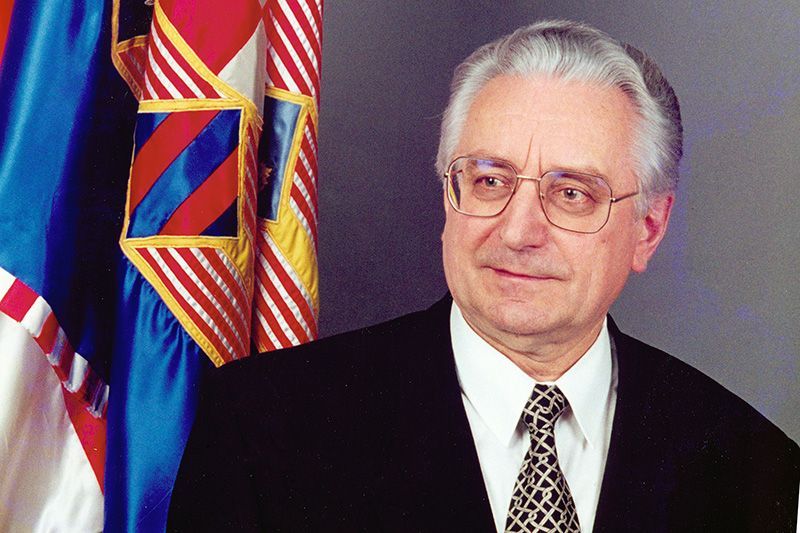
\includegraphics[width=8cm]{francek}
			\caption{History is ugly}
		\end{figure}
	\end{frame}
	
	\begin{frame}{History}
		\centering
		\textbf{OK, not that ugly.}
		\begin{figure}
			
\includegraphics[width=5cm]{jf-14}
			\vspace{1cm}
			
\includegraphics[width=5cm]{jf-15}
			\caption{Job Fair 2014 and 2015 web}
		\end{figure}
	\end{frame}

	\begin{frame}{History}
		Main guidelines
		\begin{itemize}
			\item simplify development
			\item show time and date of the event
			\item have a CV form for students
			\item maybe show the presentation timetable
			\item development from ground up every year
			\item done by a single developer in PHP and frontend stuff
		\end{itemize}
	\end{frame}

	\begin{frame}{History}
		Problems
		\begin{itemize}
			\item unsustainable - start from scratch every year
			\item lack of information
			\item no version control
			\item often edited directly in production
			\item design and usability can be improved on
		\end{itemize}
	\end{frame}

	\begin{frame}{History}
		\hspace{2cm}
		\begin{figure}
			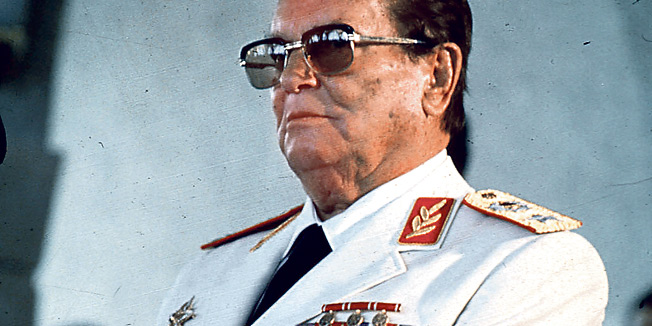
\includegraphics[width=8cm]{joza}
			\caption{Now, this is better}
		\end{figure}
	\end{frame}

	\begin{frame}{History}
		\begin{figure}
			
\includegraphics[width=8cm]{jf-17}
			\caption{Job Fair 2017 web}
		\end{figure}
	\end{frame}

	\begin{frame}{History}
		Main ideas in the beginning
		\begin{itemize}
			\item buy the design, make backend quickly
			\item still almost one pager
			\item add news section
			\item online company application
			\item use git (mind blown!)
			\item language support
			\item use rails, pgsql, slim...
		\end{itemize}
	\end{frame}

	\begin{frame}{History}
		Current state
		\begin{itemize}
			\item switched to docker
			\item added new pages (press, past, floor plan)
			\item added API for mobile
			\item dynamical company listing and timetable (modals)
			\item added a lot of information to company orders
			\item we are building a tower on top of shack foundations
		\end{itemize}
	\end{frame}

	\section{Project organization}
	
	\begin{frame}{Project organization}
		Main ideas now
		\begin{itemize}
			\item build an expandable structure
			\item organize company ux around web
			\item make mass emails and jobfair@kset.org obsolete
			\item allow easy integration of mobile and other apps
			\item start on time, don't creep the features
			\item learn agile
			\item involve more people
		\end{itemize}
	\end{frame}

	\begin{frame}{Agile / Scrum}
		\begin{figure}
			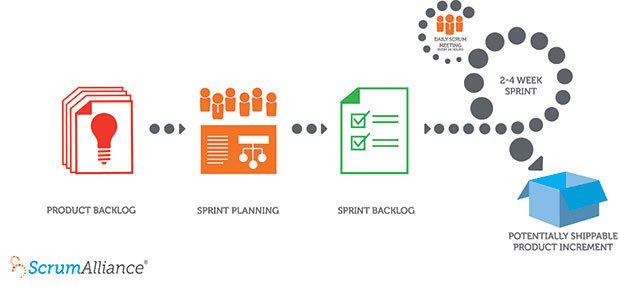
\includegraphics[width=10cm]{scrum}
			\caption{Standard Scrum workflow}
		\end{figure}
	\end{frame}

	\begin{frame}{Agile / Scrum}
		Scrum artifacts and events
		\begin{itemize}
			\item \textbf{sprint} - a given period of time (1-3 weeks)
			\item \textbf{product backlog} - contains all tasks vital for the project
			\item \textbf{sprint backlog} - tasks that will be done in given sprint
			\item \textbf{sprint planing} - periodical meeting where sprint backlog is filled and current progress is reviewed
		\end{itemize}
	\end{frame}

	\begin{frame}{Agile / Scrum}
		Scrum roles
		\begin{itemize}
			\item \textbf{product owner} - makes sure product will satisfy the client
			\item \textbf{scrum master} - makes sure team delivers on time, protects the team from greedy product owners
			\item \textbf{developer} - makes shit done :)
		\end{itemize}
	\end{frame}

	\begin{frame}{Agile / Scrum}
		How will we use it?
		\begin{itemize}
			\item Plan features in the beginning
			\item Freeze the design
			\item Split into teams
			\item Track the development progress
			\item Work hard but don't put too much stress on people
		\end{itemize}
	\end{frame}
	
	\section{Initial featureset}
	
	\begin{frame}{Features}
		\begin{figure}
			\begin{forest}
				for tree={%
				edge path={\noexpand\path[\forestoption{edge}] (\forestOve{\forestove{@parent}}{name}.parent anchor) -- +(0,-12pt)-| (\forestove{name}.child anchor)\forestoption{edge label};}
				}
				[
				Job Fair IT, calign=child,calign child=2
					[Website]
					[Business logic]
					[Mobile]
				]
			\end{forest}
			\caption{Initial project parts}
		\end{figure}
	\end{frame}

	\begin{frame}{Website}
		\begin{figure}
			\begin{forest}
				for tree={%
					edge path={\noexpand\path[\forestoption{edge}] (\forestOve{\forestove{@parent}}{name}.parent anchor) -- +(0,-12pt)-| (\forestove{name}.child anchor)\forestoption{edge label};}
				}
				[Website
					[Frontpage]
					[News]
					[Press]
					[Past editions]
					[About]
					[Impressum]
				]
			\end{forest}
		\end{figure}
	\end{frame}

	\begin{frame}{Website}
		\begin{itemize}
			\item Here to provide general info on project
			\item Attracts both companies and students
			\item Composes of basic building blocks
			\item Should be easy to manage by organization, PR, video, photo...
		\end{itemize}
	\end{frame}

	\begin{frame}{Business logic}
		\begin{figure}
			\begin{adjustbox}{width=\linewidth}
			\begin{forest}
				for tree={%
					edge path={\noexpand\path[\forestoption{edge}] (\forestOve{\forestove{@parent}}{name}.parent anchor) -- +(0,-12pt)-| (\forestove{name}.child anchor)\forestoption{edge label};}
				}
				[Business logic, calign=child,calign child=3
					[Company application]
					[Student CVs]
					[Website management]
					[User management]
					[APIs]
				]
			\end{forest}
			\end{adjustbox}
		\end{figure}
	\end{frame}

	\begin{frame}{Business logic}
		Company application
		\begin{itemize}
			\item Company applies with basic info (company name, contact info, what they want)
			\item An account manager is assigned to the company
			\item Companies get an email when they are accepted, when they have to add some info (logo, purchase order), when booth location or presentation time is assigned...
			\item All documents are stored online and are easy to access
			\item Account manager gets info when company changes info
		\end{itemize}
	\end{frame}

	\begin{frame}{Business logic}
		Student CVs
		\begin{itemize}
			\item Students can fill in their info, hide their info from certain companies, or star some companies (get reminder for presentation, tinder)
			\item Companies can view student info and search for students, view their remarks on students
			\item Automatic data extraction from pdf
			\item Integration with external applications and games?
			\item Loosen up party invitations?
		\end{itemize}
	\end{frame}

	\begin{frame}{Business logic}
		Website management
		\begin{itemize}
			\item Add/remove/edit sections
			\item Section examples: YouTube stream, gallery, call to action, news posts, testimonials, about the fair...
		\end{itemize}
		User management
		\begin{itemize}
			\item Add/remove/edit users
			\item Account managers info available to their companies
			\item Example data: name, email, phone, assigned companies, bio
		\end{itemize}
	\end{frame}

	\begin{frame}{Business logic}
		APIs
		\begin{itemize}
			\item Expose public company info
			\item Integration with mobile applications
			\item Companies can generate keys and access/add student data?
			\item Eg. company makes a game that you can access only if you have entered a CV db. It exposes your name and email to company. Game saves your top score in the game - key/value data. 
		\end{itemize}
	\end{frame}

	\begin{frame}{Features}
		\begin{figure}
			\begin{forest}
				for tree={%
					edge path={\noexpand\path[\forestoption{edge}] (\forestOve{\forestove{@parent}}{name}.parent anchor) -- +(0,-12pt)-| (\forestove{name}.child anchor)\forestoption{edge label};}
				}
				[Mobile, calign=child,calign child=2
					[For companies]
					[For students]
					[For organizers?]
				]
			\end{forest}
		\end{figure}
	\end{frame}
	
	\section{Timeline and parallel development}
	
	\begin{frame}{Project timeline}
		\begin{figure}
			\resizebox{!}{.7\textheight}{
				\begin{ganttchart}{1}{24}
					\gantttitlelist{6,7,8,9,10,11,12,1,2,3,4,5}{2} \\
					\ganttbar{Solution design}{1}{1} \\
					\ganttmilestone{Design freeze}{1} \ganttnewline
					\ganttbar{Web development}{2}{18} \ganttnewline
					\ganttbar{Backend development}{2}{18} \ganttnewline
					\ganttbar{Mobile development}{8}{18} \ganttnewline
					\ganttmilestone{Development freeze}{18} \ganttnewline
					\ganttbar{Production}{15}{23} \\
					\ganttmilestone{Event}{23} \ganttnewline
				\end{ganttchart}
			}
		\end{figure}
	\end{frame}

	\begin{frame}{Project timeline}
		Sprint organization
		\begin{itemize}
			\item Start with 1 week sprints for next 2 weeks - design discussion
			\item Hold a total of 4 team meetings and fill the backlog
			\item Have a clear picture of all product parts
			\item After that we switch to 2 week sprints
			\item Develop features by their importance - blocking first
		\end{itemize}
	\end{frame}

	\begin{frame}{Project timeline}
		During design phase
		\begin{itemize}
			\item Gather information
			\item Decide on the technology
			\item Describe user interaction
			\item Prepare database model
			\item Add features to product backlog
		\end{itemize}
	\end{frame}

	\begin{frame}{Project timeline}
		Organize teams
		\begin{itemize}
			\item Split into teams - backend, web and mobile
			\item Assign product owners and scrum masters
			\item Schedule sprint planing meetings
			\item Prepare GitHub projects
		\end{itemize}
	\end{frame}

	\begin{frame}{Project timeline}
		General priorities after design phase
		\begin{itemize}
			\item Prepare the environment - development server, GitHub, CI
			\item Find a solution how to make frontend
			\item Web backbone - simple CMS and basic sections
			\item Users, companies and students models and admin
		\end{itemize}
	\end{frame}

	\section{The goal}
	
	\begin{frame}{The goal}
		\textbf{The goal:} Create a new and shiny website which will eliminate the need for mailing lists, collect all company and student data in one place and most importantly have a stable platform that will enable future development of the whole ecosystem. Develop on time and learn/teach new technologies, development processes and concepts. Have fun and sense of self reward!
	\end{frame}
	
	\section{Surprise}
	
	\begin{frame}{Beer}
		\begin{figure}
			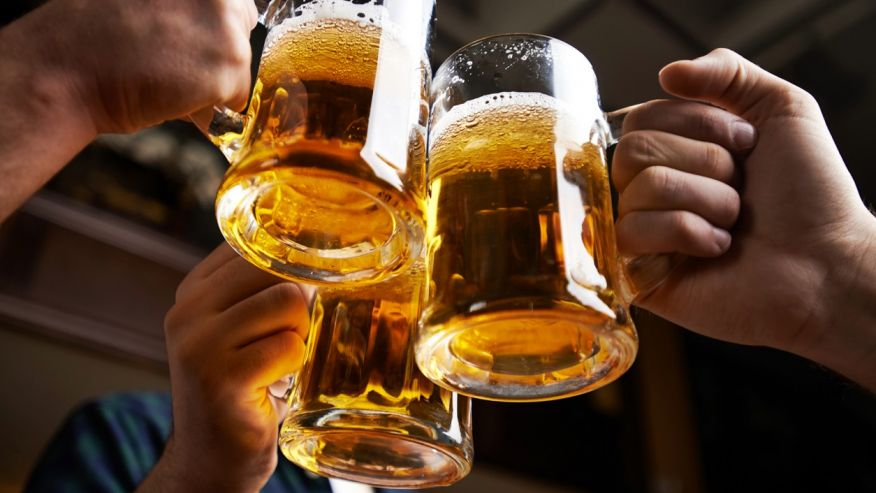
\includegraphics[width=8cm]{beer}
			\caption{Free beer every sprint planning}
		\end{figure}
	\end{frame}

	\section{Thanks}

\end{document}
